\documentclass[draft,ras]{Template/AGUTeX}

\usepackage{graphicx}   % if you want to include graphics files
\usepackage{subfigure}
\usepackage{setspace}
\usepackage{amsxtra}
\usepackage{amsmath}
\usepackage{amssymb}
\usepackage{multirow}
\usepackage{bm}
\RequirePackage{lineno}
\linenumbers
% graphics path
\graphicspath{{Figs/}}

\authorrunninghead{SWOBODA ET AL.}
\titlerunninghead{ESA ISR}


\authoraddr{Corresponding author: J. P. Swoboda,
Department of Electrical \& Computer Engineering,
Boston University, 8 Saint Mary�s Street
Boston, MA 02215, USA.
(swoboj@bu.edu)}

\begin{document}

\title{Space-Time Ambiguity Function for Electronically Scanned ISR}
%%%%%%%%%%%%%% Author Info %%%%%%%%%%%%%%%%%%%%%%%%%%%%%%%%%%%%%
\authors{John Swoboda,\altaffilmark{1}
Joshua Semeter,\altaffilmark{1} Philip Erickson \altaffilmark{2}}

\altaffiltext{1}{Department of Electrical \& Computer Engineering,
Boston University, Boston, Massachusetts, USA.}
\altaffiltext{2}{Atmospheric Science Division,
MIT Haystack Observatory, Westford Massachusetts, USA.}
%%%%%%%%%%%%%% Abstract %%%%%%%%%%%%%%%%%%%%%%%%%%%%%%%%%%%%%

\begin{abstract} Electronically steerable array (ESA) technology has recently been used in incoherent scatter radars (ISR). These arrays allow for pulse-to-pulse steering of the antenna beam to collect data in a three dimensional region. This is in direct contrast to dish based antennas where acquisition is limited to take data in a two dimensional slice. This allows for more flexibility in the measurement of ionospheric plasma parameters.  

Currently these systems are operating in the high latitude region where the ionosphere is highly dynamic in both space and time. Because of the highly dynamic nature of the ionosphere in this region it is important to differentiate between artifacts and the true behavior of the plasma. Often the three dimensional data is fitted in a spherical coordinate space and then the parameters are interpolated to a Cartesian grid. This and other sources of error could be impacting the reconstructions of the plasma parameters.

To take advantage of the new flexibility of ESA system we present a new way of analyzing ISR through use of the space-time ambiguity function. This concept is similar to the range ambiguity function that is used in traditional ISR for scanning antenna systems but has been extended to all spatial dimensions along with time as well. 

The use of this new ambiguity function allow us to pose this problem in terms of a  linear inverse problem for the lags of the intrinsic plasma autocorrelation function. From this we can explore the impact of non-uniformity in the plasma parameters in both time and space. Along with showing possible artifacts we will begin to discuss ways of reducing them and improving the quality of data products from electronically steerable ISRs.

\end{abstract}

%%%%%%%%%%%%%%  End of Abstract %%%%%%%%%%%%%%%%%%%%%%%%%%%%%%%%%%


\begin{article}

%%%%%%%%%%%%%% Intro %%%%%%%%%%%%%%%%%%%%%%%%%%%%%%%%%%%%%

\section{Introduction}
Incoherent scatter radar (ISR) is a powerful tool for exploring the ionosphere. These systems can give measurements of electron density $N_e$, ion temperature $T_i$, electron temperature $T_e$, ion velocity $V_i$ and other plasma parameters \citep{dougherty:farley1960, farleydougherty:ISR2, doughteryfarley:ISR3, hagfors1961}. These parameters are measured by fitting a nonlinear theoretic autocorrelation function (ACF) model derived from first principles physics to an estimated time autocorrelation or, alternatively, the power spectrum of the radar signal scattered off of random electron density fluctuations \citep{Lehtinen1996435}. 

This is an estimation of a second order statistic of an inherently random process of scattering from electrons. In order to get an estimate of the ACF with reasonable statistical properties numerous pulses have to be averaged together. With traditional dish antennas the ISR system would build these statistics in a limited number of ways. One method consists of pointing the radar beam in a specific direction and hold it there until enough pulses were integrated to get the desired statistics. Alternatively, the beam could be scanned through a field of view and collect pulses while moving. These techniques have an implicit assumption about the uniformity of the plasma parameters within the beam while pulses are being integrated. This leads to the assumption of the stationarity of the ACF within a temporal and spatial resolution of the radar. %The first method assumes a stationarity of the ACF in time while the pulses are collected while the second technique assumes that the velocity of the plasma is known and the beam is scanning along it's velocity or more simply that the plasma parameters, and thus the ACF, are not changing along the motion of the beam.

In many cases, especially in the high latitude ionosphere, this stationarity assumption is not met. Phenomena such as polar cap patches that may be drifting at greater than 1km/s, and thus the residency time of a particular plasma parcel within a radar beam may be much shorter than the integration time required to estimate an ACF\citep{dahlgren2012di}. In the auroral zone, ionospheric variations produced by auroral particle precipitation on similarly short time scales compared to the integration period period \citep{Zettergren:2008ba}.%Poleward Boundary intensifications also can break these assumptions due to the two dimensional structure \citep{JGRA:JGRA17576, JGRA:JGRA16190}.
%This initial work showed the nonlinear relationship between the plasma parameters and the incoherent scatter autocorrelation function. 

%As with any real world measurement method there is a limit to the spatial and temporal resolution of ISR systems. This resolution is determined by the ability of the sensor to create independent statistical estimates of the ACF in time and space of what is essentially a zero-mean complex Gaussian process. At space and time extents smaller then these resolutions the random process that the ACF is derived from is assumed to be stationary. In ISR literature the ambiguity function encapsulates the spatial resolution in the range dimension. This ambiguity emerges as a function of range and correlation lag due to the pulse modulation and the finite bandwidth of the receiver \citep{farley1969}. The time resolution is determined by how long it takes to average the autocorrelation function to reduce the variance of the estimate to a desired level.

%The hard target radar world also uses an ambiguity to analyze resolution but it is a function of time delay and Doppler mismatch. The CPI for a pulse doppler is like the time ambiguity. This ambiguity is tied to 

%This assumption of stationarity at the level of the ambiguity function constrains the measurement and creates a blurring and other forms of artifacts due to the non-linear fitting of plasma parameters. In order to reduce the impact of these ambiguities a number techniques have been developed. Some techniques include trying to reduce the extent of the ambiguity function by adjusting the waveform. Barker code wave forms are used in ISR but mainly for low altitude studies of the E-region due to the inability to form a spectrum from them. Another method for reducing the ambiguity in range is using alternating codes \citep{grayfarley:isrcomppulse, lehtinen;ac, Sultzer1993, 1989AdSpR...9..153S}. %These codes though do reduce the amount of power returned from a specific volume of plasma.

%Another set of techniques often shown in the literature focus on reducing the impact of the ambiguity function through post processing. The first method, full profile analysis, consists of fitting physical parameter values to entire range extent taking into account all of the correlations between all locations \citep{holt1992, Lehtinen1989133, Lehtinen:1997uh,hysell2008}. This technique often places constraints on the physical parameters as in \citet{hysell2008}. Because the the relationship between the autocorrelation function and the lags are non-linear this method often yields algorithms that require a large amount computation to calculate the covariance matrices between all of the values.

%The other set of post processing methods, such as in \citet{nikoukar2008} and \citet{Virtanen:2008vx}, treat the problem as a linear inverse problem of the lags. Methods such as total-variations or Tikihonov regularization can be applied to the lags to try to fill in the missing information nation from the null space of the operator. These methods are easy to compute and can rely on a large body of knowledge from engineering communities that study linear inverse problems. 

Recently electronically steerable array (ESA) technology has started to be leveraged by the ISR community. The Advance Modular Incoherent Scatter Radar (AMISR) systems have already been deployed both at the Poker Flat Alaska (PFISR) and Resolute Bay Canada (RISR) \citep{amisr.site}. The EISCAT-3D project is currently being developed using phased array technology as well and will be capable of multistatic processing \citep{eiscat3ddesign}. These new systems are already being used in a number of different ways including creating volumetric reconstructions of plasma parameters \citep{Semeter2009738, Nicolls:2007ie, dahlgren2012di,Dahlgren:2012dq}. These reconstructions mainly consist of taking ISR data after parameters have been fit in a spherical coordinate system and then interpolate them into a Cartesian space.

These new ESA based systems differentiate themselves from dish antennas in a fundamental way. Instead of dwelling in a single beam or scanning along a prescribed direction, an ESA can move to a different beam position within its field of view on a pulse by pulse basis. This yields a new flexibility to integrate different beams in such a way that the original velocity of the plasma can be unknown. This can help to relax the assumption of stationarity in that now the plasma can move into a different beam and have the returns from the same plasma be integrated together. As opposed to the case with a dish antenna where the returns from different plasma would be improperly averaged together.

In order to take advantage of this new flexibility this work puts forth the idea of the space-time ambiguity function. This concept extends the range ambiguity to all three spatial dimensions along with time. The goal of this paper is to develop the formalism for treating space-time ambiguity for electronically steerable ISRs or ISRs that are capable of sampling a given volume on a pulse-by-pulse basis. The impact of the three-dimensional ambiguity on moving plasma will be shown through specific cases related to the polar cap patches. A simulation of a polar cap patch using a full ISR simulator, which creates ISR data at the I/Q level, will be shown. Lastly we will explore a number of different ways that could improve measurements from electronically steerable ISR systems.

%There has been no formal derivation of an ambiguity function for all three spatial dimensions for these systems, although up until recently ISR systems, which only had dish antennas, could not mitigate the finite beam width effects. In a highly dynamic region like the high latitude ionosphere this lack of knowledge can be problematic. There are numerous phenomena such as polar cap patches that may be moving through the field of view at very high speeds \citep{dahlgren2012di}. This motion can cause an apparent expansion in the shape of the beams if one represents the beams in the frame of reference of the moving plasma.

%These three-dimensional reconstructions often consist of taking the fitted parameters and then interpolating them to a Cartesian space from the system's natural spherical coordinate space \citep{Butler:2013ul}. The step of fitting the autocorrelation function to the theoretical functions to find the final plasma parameters is a non-linear operation. Because of this it is impossible to exactly predict the impact on the parameter values as different plasma populations move through the field of view of the radar. Alternatively it is possible to treat the formation of the autocorrelation estimates as a linear process with each lag as an independent channel \citep{nikoukar2008}.


%In this publication we will develop a model for a full three dimensional space-time ambiguity function for 3-D ISR systems. This function can also be modified to show the ambiguity within the rest frame of the moving plasma. In the end this full three dimensional can be represented as kernel in a Fredholm integral equation,

%\begin{equation}
%\label{eqn:friedholm}
%\rho(\mathbf{r}_{s}) = \int K(\mathbf{r}_{s},\mathbf{r}) R(\mathbf{r}) d\mathbf{r}
%\end{equation}

%\noindent where, for ISR, $R(\mathbf{r}))$ is the lag of the autocorrelation function at a specific time and position.
%In this publication we will describe a model for the full space-time ambiguity function for ISR systems. The impact of the three-dimensional ambiguity on moving plasma will be shown through specific cases related to the polar cap patches. A simulation of a polar cap patch using a full ISR simulator, which creates ISR data at the IQ level, will be shown. Lastly possible mitigation techniques will be explored. %These mitigation techniques will borrow heavily from the image and signal processing literature.


%%%%%%%%%%%%%% Ambiguity Derivation%%%%%%%%%%%%%%%%%%%%%%%%%%%%%%%

\section{Space-Time Ambiguity}

The space-time ambiguity can be thought of as a kernel to a combined volume and time integration operator. In the end this ambiguity can be represented as kernel in a Fredholm integral equation,

\begin{equation}
\label{eqn:friedholm}
\rho(\mathbf{r}_{s}) = \int K(\mathbf{r}_{s},\mathbf{r}) R(\mathbf{r}) d\mathbf{r}
\end{equation}

\noindent where, for ISR, $R(\mathbf{r})$ is the lag of the autocorrelation function at a specific time and position.

By using this formulation many parallels between ISR and classic camera blurring problems can be made. In cameras blurring can take place when an object moves over a space covered by one pixel while the shutter is open and the CCD is collecting photons. A diagram of this can be seen in Figure \ref{fig:ccd}. The same holds for ISR except that the pixels are no longer square and instead are determined by the beam shape and pulse pattern. This is shown in the diagrams in Figure \ref{fig:radarblur}.

\begin{figure}[h!]
    \centering
    \subfigure[CCD No Blur]{
        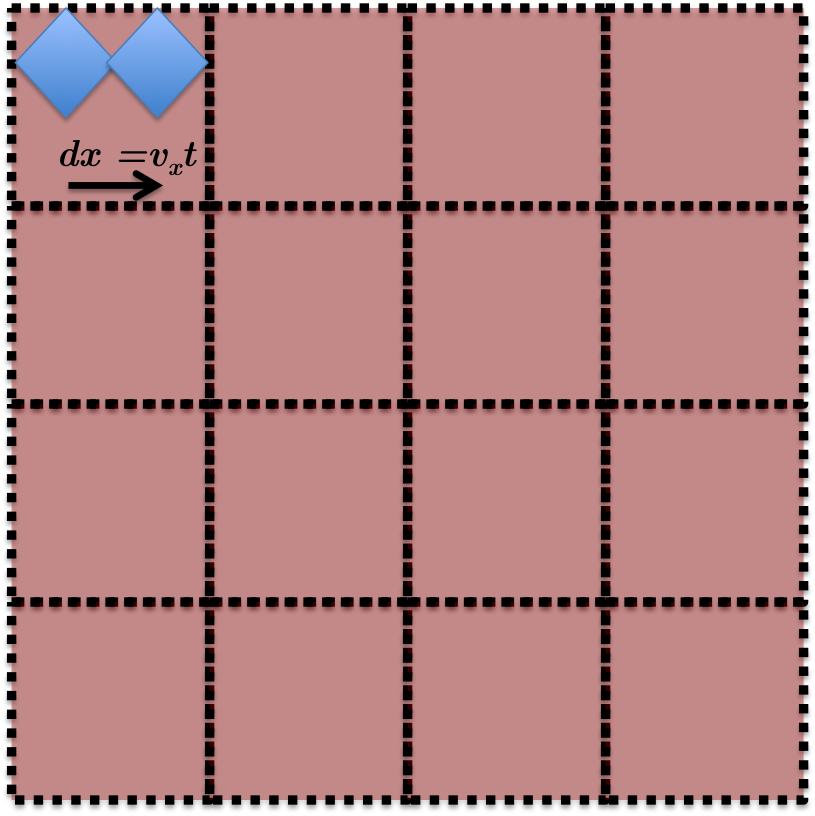
\includegraphics[height=2in]{ccddiagramnoblur}
        \label{sfig:ccdnoblur}}
    \quad
    \subfigure[CCD With Blur]{
        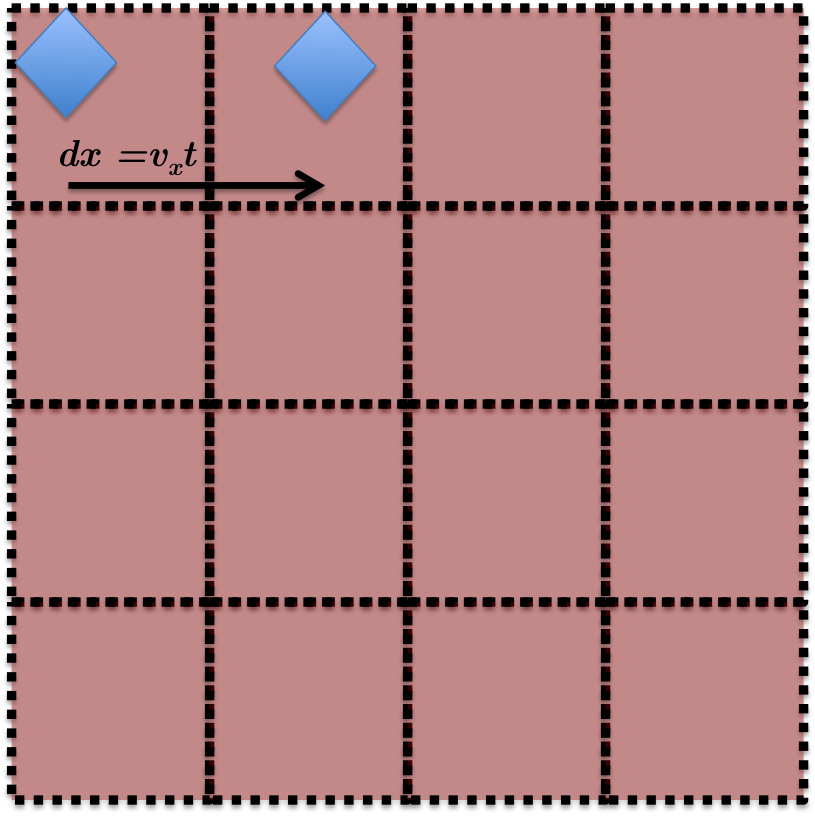
\includegraphics[height=2in]{ccddiagramblur}
        \label{sfig:ccdblur}}
    \caption{CCD camera}
    \label{fig:ccd}
\end{figure}

\begin{figure}[h!]
    \centering
    \subfigure[Radar No Blur]{
        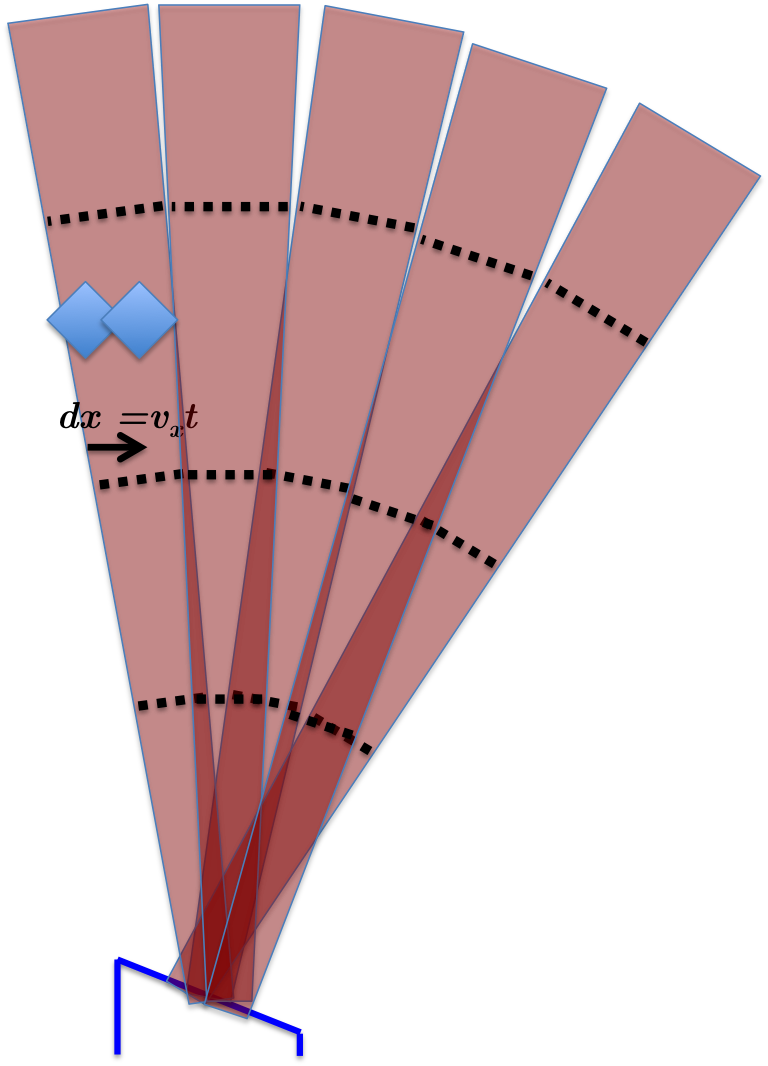
\includegraphics[height=2in]{radardiagramnoblur}
        \label{sfig:radarnoblur}}
    \quad
    \subfigure[Radar With Blur]{
        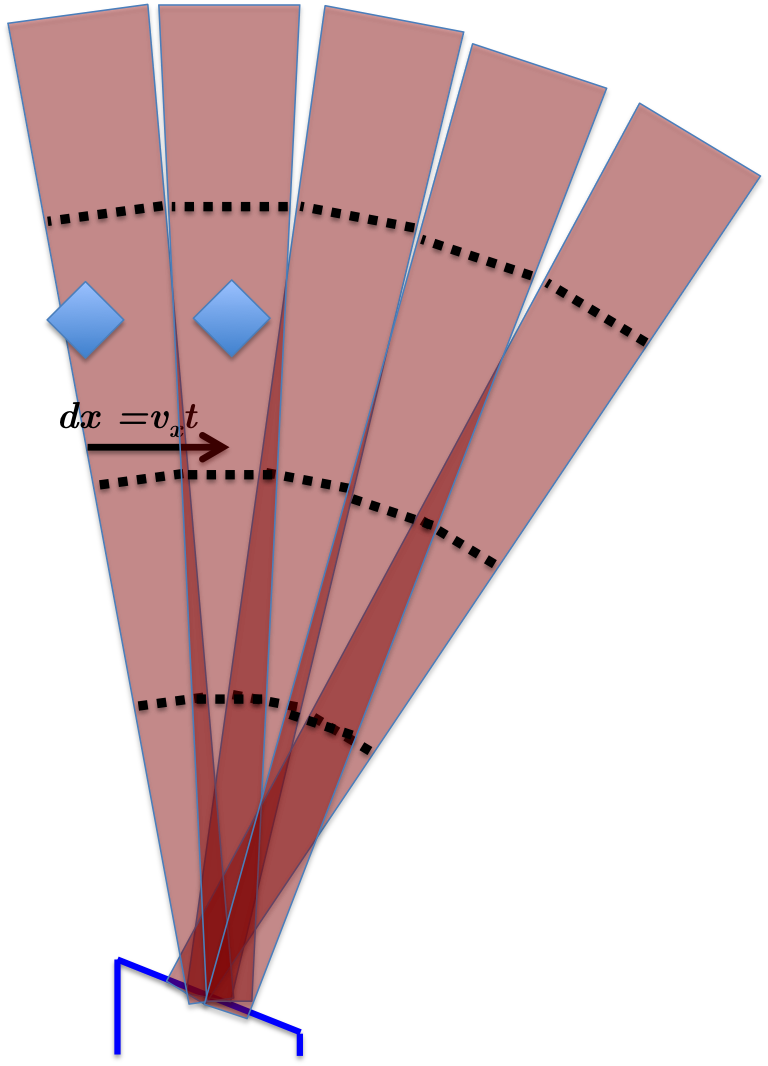
\includegraphics[height=2in]{radardiagramblur}
        \label{sfig:radarblur}}
    \caption{Radar}
    \label{fig:radarblur}
\end{figure}
Before we derive this ambiguity function we will start with defining our coordinate system.

\subsection{Coordinate System Definitions}

Our three dimensional coordinate system is defined as $\mathbf{r}=[x,y,z]^T$. For this coordinate system, $\mathbf{r}=[0,0,0]^T$ at the location of the radar and thus $r=|\mathbf{r}|$, also known as the range variable. This allows for the use of polar coordinates $\mathbf{r} =  [r,\theta_,\phi]^T$ where $\theta$ is the physical elevation angle, $\phi$ is the physical azimuth angle.

The radar will sample this space into a set of discrete points which will be referred to as $\mathbf{r}_s = [x_s,y_s,z_s]^T$ along with the discretized range $r_s=|\mathbf{r}_s|$. The sampled space will consist of a number of points which are the combinations of range gates and number of beams. These points can also be referred in the polar coordinates $\mathbf{r}_s = [r_s,\theta_s,\phi_s]^T$, where $\theta_s$ is the sampled elevation angle, $\phi_s$ is the sampled azimuth angle.

For notation purposes we use two different sets of time commonly known in radar literature as fast-time, $n$ and slow-time, $t$ \citep{richards:fundamentalsigproc}. Fast-time is used to describe processes with correlation time less then one pulse repetition interval (PRI). Slow-time will be used for processes that decorrelate in time on the order of the system's PRI. In order to form estimates of the ACFs, with desired statistical properties, it is assumed that the plasma parameters parameters will change on the order of many tens to hundreds of PRIs in their stationary reference frame. Generally for incoherent scatter the in the E-region of the ionosphere and above the decorrelation time is less then a PRI, thus the ACFs are formed over fast-time.

The terms $n$ and $t$ will represent a continuous variables while $n_s$ and $t_s$ will be the fast time and slow time parameters sampled by the radar. The sampling rate of $n_s$ will be that of the A/D converters. The sampling of $t_s$ can at the highest rate, be the PRI. At it's lowest, it can be  sampled once in a non-coherent processing interval (NCPI), or a period of time it takes the radar to average the desired number of pulses. 

%In the ISR literature the measurement ambiguity along the range dimension is often referred to simply as the ambiguity function \citep{hysell2008}. This only shows the measurement ambiguity along the range $r$. Due to the three-dimensional imaging capability of phased array ISR systems we will define a new set of terminology to describe this more complicated measurement which is now imaging the ionosphere in three-dimensional continuous coordinates $\mathbf{r}=[x,y,z]^T$. This coordinate system $\mathbf{r}=[0,0,0]^T$ at the location of the radar. The radar will create a 3-D representation of the ionospheric parameters in to discrete coordinates $\mathbf{r}_s = [x_s,y_s,z_s]^T$.

%Specifically we will refer to the measurement ambiguity in the range dimension as the range ambiguity, $W(\tau,r_s,r)$. The measurement ambiguity in the elevation and azimuth angles will be referred to as the angular or cross range ambiguity $F(\theta_s,\phi_s,\theta,\phi)$, where $\theta$ is the physical elevation angle, $\phi$ is the physical azimuth angle, $\theta_s$ is the elevation angle that the radar is pointing at and $\phi_s$ is the azimuth angle that the radar is pointing at. The since these two functions are separable they can be multiplied together to form the full spatial ambiguity $K(\tau,\mathbf{r},\mathbf{r}_s)$. Lastly integration time for each measurement will be referred to the time ambiguity. Again like the full spatial ambiguity function we can multiply the space and time ambiguity functions to get the Space-Time ambiguity function which will be represented as $L(\tau,\mathbf{r}_s,t_s,\mathbf{r},t)$ .% Might want to go through math from the kernel stuff.

\subsection{Derivation}

The basic physical mechanism behind ISR is that electron density fluctuations in the ionosphere, $n_e(\mathbf{r},n)$, scatter radio waves which can be observed by the receiver system of the radar \citep{dougherty:farley1960}. The emitted radar signal at the transmitter will have a pulse shape $s(n)$ modulated at a central frequency that results in a scattering wave number $\mathbf{k}$. Using the Born approximation the signal received at time $n$, $x(n)$, can be represented as the following

\begin{equation}
\label{eq:xt}
x(n) = h(n) \ast \int e^{-j\mathbf{k} \cdot \mathbf{r}}  s\left(n-\frac{2r}{c}\right) n_e(\mathbf{r},n) d\mathbf{r},
\end{equation}

\noindent where $h(n)$ is the receiver filter and the $\ast$ represents the convolution operator. In modern ISR systems this signal $x(n)$ is then sampled at discrete points in fast-time which will be referred to as $n_s$. The convolution and sampling operation can be brought in the integral as the following,

\begin{equation}
\label{ex:xtaug}
x(n_s) = \int e^{-j\mathbf{k} \cdot \mathbf{r}}  s\left(n-\frac{2r}{c}\right) n_e(\mathbf{r},n)h(n_s-n) d\mathbf{r}dn
\end{equation}


Once the signal has been received and sampled the autocorrelation function is then estimated from the sampled signal $x(n_s)$. The full expression of the underlying autocorrelation of this signal is the following, 

\begin{multline}
\label{ex:acf0}
\langle x(n_s)x^*(n_s')\rangle =  \int e^{-j \mathbf{k}\cdot \left(\mathbf{r}'-\mathbf{r} \right)}s\left(n-\frac{2r}{c}\right)s^*\left(n'-\frac{2r'}{c}\right) \\ h(n_s-n)h(n_s'-n')\langle n_e(\mathbf{r},n)n^*_e(\mathbf{r}',n')\rangle d\mathbf{r} d\mathbf{r}'dn dn',
\end{multline}

\noindent where $r'$ is the magnitude of the vector $\mathbf{r}'$. By assuming stationarity of second order signal statistics along fast time, we can then substitute the the lag variables $\tau\equiv n'-n$, and $\tau_s\equiv n_s'-n_s$. With these substitutions Equation \ref{ex:acf0} becomes


\begin{multline}
\label{ex:acf1}
\langle x(n_s)x^*(n_s+\tau_s)\rangle =\int e^{-j \mathbf{k}\cdot \left(\mathbf{r}'-\mathbf{r} \right)}s\left(n-\frac{2r}{c}\right)s^*\left(n+\tau-\frac{2r'}{c}\right) \\ h(n_s-n)h(n_s+\tau_s-n-\tau) \langle n_e(\mathbf{r},n)n^*_e(\mathbf{r}',n+\tau)\rangle d\mathbf{r} d\mathbf{r}' dnd\tau
\end{multline}

\noindent We can make a simplifying assumption at this point that the space-time autocorrelation function of $n_e(\mathbf{r},t)$, $\langle n_e(\mathbf{r},n)n_e(\mathbf{r}',n+\tau)\rangle$, will go to zero as the magnitude of $\mathbf{y} \equiv \mathbf{r}'-\mathbf{r}$ increases beyond the debye length\citep{farley1969}. Thus, the rate which the spatial autocorrelation goes to zero will be such that $\tau\gg \frac{2||\mathbf{y}||}{c}$  allowing us to set $r= r'$. This allows Equation \ref{ex:acf1} to be rewritten as 
 
 \begin{multline}
 \label{ex:acf2}
 \langle x(n_s)x^*(n_s+\tau)\rangle = \int s\left(n-\frac{2r}{c}\right)s^*\left(n+\tau -\frac{2r}{c}\right) h(n_s-n)h^*(n_s+\tau_s-n-\tau) \\\left[\int e^{-2j \mathbf{k}\cdot \mathbf{y}} \langle n_e(\mathbf{r},n)n^*_e(\mathbf{y}+\mathbf{r},n+\tau)\rangle d\mathbf{y} \right]d\mathbf{r}dn d\tau.
 \end{multline}

The inner integral is a spatial Fourier transform evaluated at the wave number of the radar $\mathbf{k}$. By again asserting stationarity along slow time we can represent the true ACF as the following,
 \begin{equation}
 \label{eq:spft}
R(\tau,\mathbf{r})= \langle |n_e(\mathbf{k},r,\tau)|^2\rangle \equiv  \int e^{-2j \mathbf{k}\cdot \mathbf{y} } \langle n_e(\mathbf{r},b)n^*_e(\mathbf{y}+\mathbf{r},n+\tau)\rangle d\mathbf{y}.
 \end{equation}
 
 \noindent Now Equation \ref{ex:acf2} becomes
 
 \begin{equation}
 \langle x(n_s)x^*(n_s+\tau_s)\rangle = \int \langle |n_e(\tau,\mathbf{k},\mathbf{r})|^2\rangle\left[\int s(n-\frac{2r}{c})s^*(n+\tau -\frac{2r}{c})h(n_s-n)h^*(n_s+\tau_s-n-\tau) dn \right]d\tau dr.
 \end{equation}

 If $n_s$ is replaced with $2r_s/c$ we can introduce the range ambiguity function $W(\tau_s,r_s,\tau,r)$ by doing the following substitution,
 \begin{equation}
 \label{eqn:rngamb}
 W(\tau_s,r_s,\tau,r)= \int s(n-\frac{2r}{c})s^*(n+\tau -\frac{2r}{c})h(2r_s/c-n)h^*(2r_s/c+\tau_s-n-\tau) dn.
 \end{equation}
 
Assuming, for the moment, that $R(\tau,\mathbf{r})$ only varies across the range dimension $r$ we can now represent this in the form of a Fredholm integral equation
 
 \begin{equation}
 \label{eqn:fredfirst}
 \langle x(2r_s/c)x^*(2r_s/c+\tau_s)\rangle = \int W(\tau_s,r_s,\tau,r)R(\tau,r) drd\tau.
 \end{equation}
 
\noindent The range ambiguity function, $W(\tau_s,r_s,\tau,r)$, can be thought of as a smoothing operator along the range and lag dimensions of $R(\tau,r)$. 

%% Old stuff 
 
 
 
%Recently some publications have assumed the bandwidth of the receiver was much larger then the bandwidth of the fluctuations in electron density thus it can be assumed that filter will only act on the the shape of the pulse\citep{nikoukar2008}. Others though take impact of the receiver filter into
%This will change Equation \ref{eq:xt} to the following:
%
%\begin{equation}
%\label{ex:xtaug}
%x(n) = \int_{\mathbf{r}} e^{-j\mathbf{k} \cdot \mathbf{r}}  a\left(n-\frac{2r}{c}\right) n_e(\mathbf{r},n) d\mathbf{r}
%\end{equation}
%\noindent where $a(n)= h(n) \ast s(n)$.   
%
%
%\noindent where $r'$ is the magnitude of the vector $\mathbf{r}'$. 
%
%
%If we assume stationarity of the second order statistic of the signal along fast time $n$ we can substitute a lag variable $\tau\equiv n'-n$, Equation \ref{ex:acf0} becomes
%
%
%When the autocorrelation of the signal is done we find the following formula, \citep{nikoukar2008},
%
%\begin{equation}
%\label{ex:acf0}
%\langle x(n)x^*(n')\rangle = \int_{\mathbf{r'}}\int_{\mathbf{r}} e^{-j \mathbf{k}\cdot \left(\mathbf{r}'-\mathbf{r} \right)}a\left(n-\frac{2r}{c}\right)a^*\left(n'-\frac{2r'}{c}\right) \langle n_e(\mathbf{r},n)n^*_e(\mathbf{r}',n')\rangle d\mathbf{r} d\mathbf{r}'
%\end{equation}
%
%\noindent where $r'$ is the magnitude of the vector $\mathbf{r}'$. If we assume stationarity of the second order statistic of the signal along fast time $n$ we can substitute a lag variable $\tau\equiv n'-n$, Equation \ref{ex:acf0} becomes
%
%\begin{equation}
%\label{ex:acf1}
%\langle x(n)x^*(n+\tau)\rangle = \int_{\mathbf{r'}}\int_{\mathbf{r}} e^{-j \mathbf{k}\cdot \left(\mathbf{r}'-\mathbf{r} \right)}a\left(n-\frac{2r}{c}\right)a^*\left(n+\tau-\frac{2r'}{c}\right) \langle n_e(\mathbf{r},n)n^*_e(\mathbf{r}',n+\tau)\rangle d\mathbf{r} d\mathbf{r}'.
%\end{equation}
% 
%\noindent We can make a simplifying assumption at this point that the space-time autocorrelation function of $n_e(\mathbf{r},t)$, $\langle n_e(\mathbf{r},n)n_e(\mathbf{r}',n+\tau)\rangle$, will go to zero as the magnitude of $\mathbf{y} \equiv \mathbf{r}'-\mathbf{r}$ increases. The rate that the space-time autocorrelation goes to zero will be such that $\tau\gg \frac{2||\mathbf{y}||}{c}$ thus in the argument of the pulse shape $r\approx r'$. This allows Equation \ref{ex:acf1} to be rewritten as 
% 
% \begin{equation}
% \label{ex:acf2}
% \langle x(n)x^*(n+\tau)\rangle = \int_{\mathbf{r}} a\left(n-\frac{2r}{c}\right)a^*\left(n+\tau -\frac{2r}{c}\right) \int_{\mathbf{y}} e^{-2j \mathbf{k}\cdot \mathbf{y}} \langle n_e(\mathbf{r},n)n^*_e(\mathbf{y}+\mathbf{r},n+\tau)\rangle d\mathbf{y} d\mathbf{r}.
% \end{equation}
% 
% The inner integral is a spatial Fourier transform evaluated at the wave number of the radar $\mathbf{k}$
% \begin{equation}
% \label{eq:spft}
% \langle |n_e(\mathbf{k},r,\tau)|^2\rangle \equiv  \int_{\mathbf{y}} e^{-2j \mathbf{k}\cdot \mathbf{y} } \langle n_e(\mathbf{r},b)n^*_e(\mathbf{y}+\mathbf{r},n+\tau)\rangle d\mathbf{y}.
% \end{equation}
% 
% \noindent Now Equation \ref{ex:acf2} becomes
% 
% \begin{equation}
% \langle x(n)x^*(n+\tau)\rangle = \int_{r} a(n-\frac{2r}{c})a^*(n+\tau -\frac{2r}{c}) \langle |n_e(\tau,\mathbf{k},\mathbf{r})|^2\rangle dr.
% \end{equation}
% %angle ambiguity
% %E_e(\phi,\psi)\text{dirc}_N(\frac{d_1}{\lambda}\sin\phi \cos\psi)\text{dirc}_K\left(\frac{d_2}{\lambda}\sin\phi\sin\psi\right)
% %It should be noted that the term $ a(n)a^*(n+\tau)$ is the soft target ambiguity function.  
% If $n$ is replaced with $2r_s/c$ we can introduce the range ambiguity function $W(\tau,r_s,r)$ by doing the following substitution \citep{nikoukar:thesis},
% \begin{equation}
% \label{eqn:rngamb}
% W(\tau,r_s,r)= a\left(\frac{2(r_s-r)}{c}\right)a^*\left(\frac{2(r'-r)}{c}+\tau\right).
% \end{equation}
% 
% In order to simplify notation we will represent $ \langle |n_e(\tau,\mathbf{k},\mathbf{r})|^2\rangle$, as $R(\tau,\mathbf{r})$. Assuming, for the moment, that $R$ only varies across the range dimension $r$ we can now represent this in the form of a Fredholm integral equation
% 
% \begin{equation}
% \label{eqn:fredfirst}
% \langle x(2r_s/c)x^*(2r_s/c+\tau)\rangle = \int_{r} W(\tau,r_s,r) R(\tau,r) dr.
% \end{equation}
% 
%\noindent The ambiguity in the end $W(\tau,r_s,r)$ is a lag dependent smoothing along the range dimension of $R(\tau,r)$. 
%% end of old stuff
 
The spatial ambiguity across the azimuth and elevation angles is determined by the antenna beam pattern. In phased array antennas this beam pattern is ideally the array factor multiplied by the element pattern \citep{Balanis:2005:ATA:1208379}. The array factor is determined by a number of things including the element spacing and the wave number of the radar, $k$. For example, by making idealized assumptions with no mutual coupling and that the array elements are cross dipole elements, AMISR systems will have the following antenna pattern for pointing angle ($\theta_s,\phi_s$), \footnote{I could change this to a general phase array antenna pattern.}
 % make appendix to develop this further.
 \begin{equation}
 \label{eqn:amisrpat}
F(\theta_s,\phi_s,\theta,\phi) = \frac{1}{2}(1+\cos(\theta)^2)\left[ \frac{1}{MN} \left(1+e^{j(\psi_y/2 + \psi_x)}\right)\frac{\sin((M/2) \psi_x)}{\sin(\psi_x)} \frac{\sin((N/2) \psi_x)}{\sin(\psi_x/2)}\right]^2,
 \end{equation}
 
 \noindent where $\psi_x = -k d_x(\sin\theta\cos\phi-\sin\theta_s\cos\phi_s)$, $\psi_y = -k d_y(\sin\theta\sin\phi-\sin\theta_s\sin\phi_s)$ and $M$ is the number of elements in the $x$ direction of the array, and $N$ is the number of elements in the $y$ direction(see Appendix: \ref{App:AMISRarr} for derivation).


The spatial ambiguity is a separable function made up of the components of $W(\tau_s,\tau,r_s,r)$ and $F(\theta_s,\phi_s,\theta,\phi)$. These two functions can be combined by multiplying the two, creating the spatial ambiguity function  $K(\tau_s,\mathbf{r}_s,\tau,\mathbf{r})$, and then doing a volume integration. This yields an estimate of the ACF using only one pulse, which will be referred to as $\rho(\tau_s,\mathbf{r}_s)$,

 %\begin{equation}

 \begin{align}
  \label{eqn:volume}
\rho(\tau_s,\mathbf{r}_s) &= \int F(\theta_s,\phi_s,\theta,\phi)W(\tau_s,r_s,\tau,r) R(\tau,\mathbf{r}) dV,\\
	&= \int K(\tau_s,\mathbf{r}_s,\tau,\mathbf{r}) R(\tau,\mathbf{r})dV.
\end{align}
 %\end{equation}
A rendering of an example of this full spatial ambiguity function for an uncoded long pulse and antenna pattern in Equation \ref{eqn:amisrpat} for four beams can be seen in Figure \ref{fig:amb4}.

\begin{figure}
	\centering
	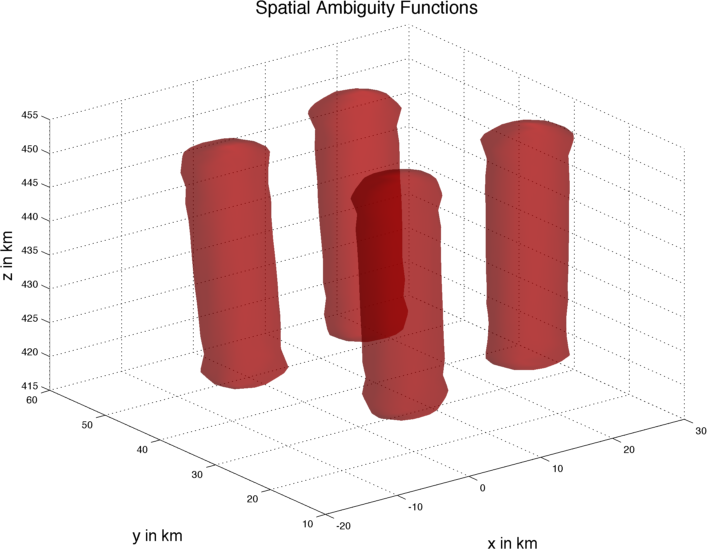
\includegraphics[width=5.5in]{spaceamb}
	\caption{Full spatial ambiguity function}	
	\label{fig:amb4}
\end{figure}

This one pulse ACF estimate represents a single sample of a random process. In order to create a usable estimate, multiple samples of this ACF need to be averaged together to reduce the variance to sufficient levels in order to fit the estimate to a theoretical ACF that is tied to plasma parameter values. To show the impact of this averaging to create the estimate of the ACF we will add slow-time dependence to $R(\tau,\mathbf{r},t)$ along with another separable function $G(t_s,t)$ to the kernel. This function $G(t_s,t)$, can be thought of as a sampling and blurring kernel for the ACF if the plasma parameters change with in an NCPI. Since the amount of time that the radar pulse is illuminating the plasma in a point of space is very short compared to IPP, $G(t_s,t)$ can take the form of a summation of Dirac delta functions 

\begin{equation}
\label{eqn:Gexp}
G(t_s,t) = \displaystyle \sum_{j=0}^{J-1}\alpha_j \delta(t-t_s-jT_{PRI}),
\end{equation}

\noindent where $J$ is the number of pulses used over a NCPI, $T_{PRI}$ is the PRI time period and $\alpha_j$ is the weights that the radar assigns to the pulses. The weights are generally set to $1/J$ to simply average the pulses. With Equation \ref{eqn:Gexp} incorporated into the overall ambiguity we see the full integral equation,

\begin{equation}
\label{eqn:sptamb}
%\rho(\tau_s,\mathbf{r}_s,t_s) &= \int G(t_s,t)K(\tau_s,\mathbf{r}_s,\tau,\mathbf{r})R(\tau,\mathbf{r},t) dV dt\\
	\rho(\tau_s,\mathbf{r}_s,t_s) =\int L(\tau_s,\mathbf{r}_s,t_s,\tau,\mathbf{r},t)R(\tau,\mathbf{r},t)dVdt.%\\
	%L(\tau,\mathbf{r}_s,t_s,\mathbf{r},t) &= G(t_s,t)F(\theta_s,\phi_s,\theta,\phi)W(\tau,r_s,r)
\end{equation}

\noindent The final kernel, $L(\tau_s,\mathbf{r}_s,t_s,\tau,\mathbf{r},t) = G(t_s,t)K(\tau_s,\mathbf{r}_s,\tau,\mathbf{r})$ encompasses the full space-time ambiguity.

\subsection{Ambiguity after Frame Transformation}

We will now focus on the impact of the motion of plasma as it is going through the field of view of the radar. We will assume that the radar is integrating over a length of time $T$ beginning at $t_s$. The kernel $L$ will be represented as a separable function $K$ and $G$ as in Equation \ref{eqn:sptamb}. In this case $G$ will be a summation of Dirac delta functions with weights of $1/J$. This will change Equation \ref{eqn:sptamb} to the following,

\begin{equation}
\label{eqn:L2}
\rho(\tau_s,\mathbf{r}_s,t_s) = \int K(\tau_s,\mathbf{r}_s,\tau,\mathbf{r}) \left[(1/J)\int_{t_s}^{t_s+T} \displaystyle \sum_{j=0}^{J-1} \delta(t-t_s-jT_{PRI})R(\tau,\mathbf{r},t) dt\right] dV.
\end{equation}

Of specific interest are instances in the high latitude ionosphere where embedded plasma structures are moving due to the electric field of the magnetosphere. Because of this it will be assumed that the plasma is a rigid object and will not deform with respect to $\mathbf{r}$ over time period $[t_0,t_0+T]$ where $T=JT_{PRI}$ is the time for one NCPI. Also it will be assumed that it will be moving with a constant velocity $\mathbf{v}$. Thus $R(\tau,\mathbf{r},t)\Rightarrow R(\tau,\mathbf{r}+\mathbf{v}t)$. The assumption of rigidity is possible to make over the time period of the NCPI, on the order of a few minutes, while the plasma moves through the field of view of the radar. One example can be taken from the high latitude ionosphere while large scale features in structures such as patches decay on the order of hours\citep{Tsunoda:1988ul}. This assumption is useful because it shows the utility of this frame work to analyze the impacts on the true resolution of the ISR systems. With these assumptions Equation \ref{eqn:L2} becomes,

\begin{equation}
\label{eqn:L3}
\rho(\tau_s,\mathbf{r}_s,t_s) =(1/J) \int \int_{t_s}^{t_s+T} \displaystyle \sum_{j=0}^{J-1}\delta(t-t_s-jT_{PRI}) K(\tau_s,\mathbf{r}_s,\tau,\mathbf{r})R(\tau,\mathbf{r}+\mathbf{v}t)dtdV\end{equation}

A change of variables to $\mathbf{r}' = \mathbf{r}+\mathbf{v}t$ acts as a Galilean transform and applies a warping to the kernel, changing the frame of reference. Since $R(\tau,\mathbf{r}')$ is no longer dependent on $t$ Equation \ref{eqn:L3} becomes,

\begin{equation}
\label{eqn:L5}
\rho(\tau_s,\mathbf{r}_s,t_s)= (1/J)\int \left[ \;\;  \displaystyle \sum_{j=0}^{J-1} K(\tau_s,\mathbf{r}_s,\tau,\mathbf{r}'-\mathbf{v}(t_s+jT_{PRI})) \;\; \right]R(\tau,\mathbf{r}')dV.
\end{equation}

By performing the integration in $t$ the problem can now be simplified further back to a Fredholm integral equation by simply replacing the terms in the square brackets as a new kernel $A(\tau_s,\mathbf{r}_s,t_s,\tau,\mathbf{r}')$,

\begin{equation}
\label{eqn:L6}
\rho(\tau_s,\mathbf{r}_s,t_s)= \int A(\tau_s,\mathbf{r}_s,t_s,\tau,\mathbf{r}') R(\tau,\mathbf{r}')dV.
\end{equation}

\noindent The impact of the plasma velocity on the ambiguity function can be seen in Figure \ref{fig:ambtime}. This is the same ambiguity as seen in Figure \ref{fig:amb4} but with a velocity of 500 m/s in the $y$ direction over a period of 2 minutes. This velocity creates a larger ambiguity function in the frame of reference of the moving plasma.
\begin{figure}[!t]
	\centering
	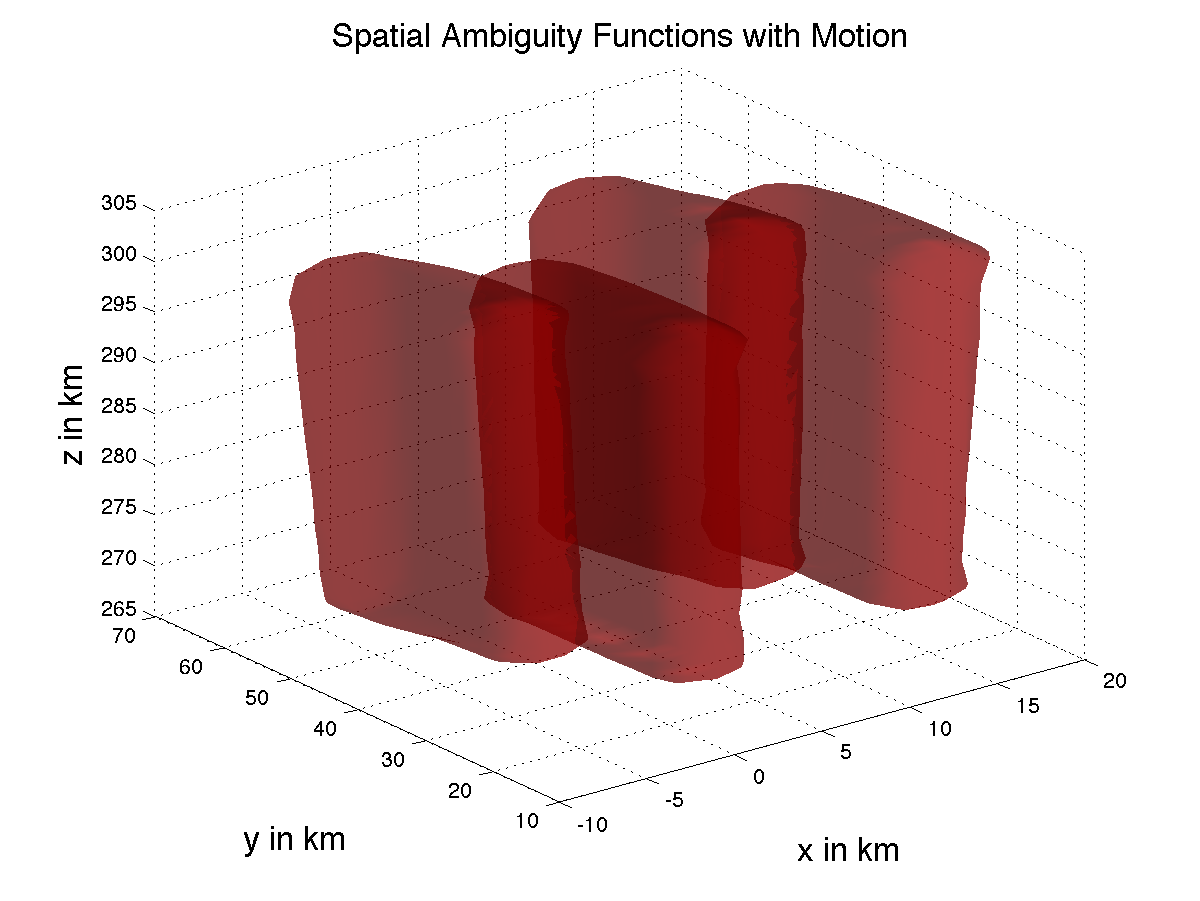
\includegraphics[width=5.5in]{spaceambmoving}
	\caption{Full spatial ambiguity function with target motion}
	\label{fig:ambtime}
\end{figure}

The operator $A$ can be determined through knowledge of the radar system's beam pattern along with the experiments pulse pattern, integration time and velocity of the plasma. This velocity $\mathbf{v}$ can be estimated by taking measurements of the Doppler shift and using a methodology seen in \citet{butler:imagingfregiondrifts}. Once the operator has been determined standard processing techniques can be used as if the plasma is not moving, under the previous assumptions.%debluring methods can be applied.

%%%%%%%%%%%%%% Simulation %%%%%%%%%%%%%%%%%%%%%%%%%%%%%%%%%%%%%

\section{Simulation}

Although Figures \ref{fig:amb4} and \ref{fig:ambtime} show the spatial extent of the space-time ambiguity function both with and without target motion, the impact of this on the reconstruction data can better shown through simulation. To do so we show data from a 3-D ISR simulator with a known ionosphere. In the following section we describe this simulator along with two case studies to show the impact of this ambiguity on properly reconstructing the parameters in the ionosphere.

\subsection{Simulator}
The simulator creates data by deriving time filters from the autocorrelation function and applying them to complex white Gaussian noise generators. Stating this in another way, every point in time and space has a noise plant and filter structure as in Figure \ref{fig:IQdiagram}. The data is then scaled and summed together according to its location in range and angle space to radar. For this simulation the data points are only used if they are within 1.1 $^\circ$ of the center beam which is a simplification of the AMISR beam pattern. 

\begin{figure}[h!]
\centering
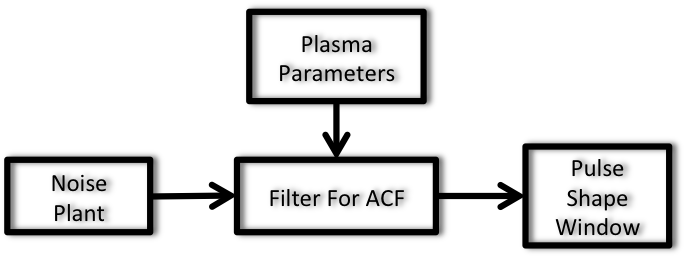
\includegraphics[width=3in]{diagrampart}
\caption{I/Q simulator diagram}
\label{fig:IQdiagram}
\end{figure}

After the IQ data has been created it is processed to create estimates of the ACF at desired points of space. This processing a follows flow chart seen in Figure \ref{fig:chain}.

\begin{figure}[!t]
\centering
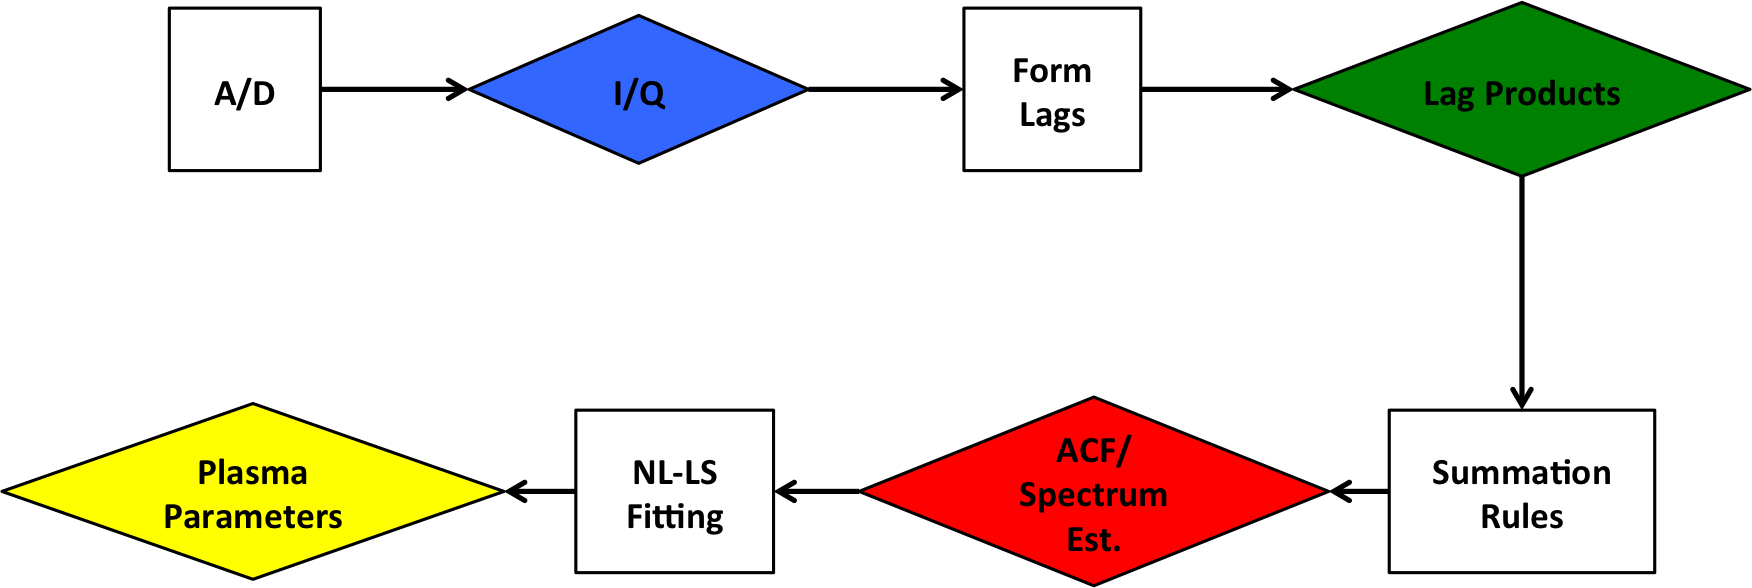
\includegraphics[width=6in]{datastackchain}
% where an .eps filename suffix will be assumed under latex, 
% and a .pdf suffix will be assumed for pdflatex; or what has been declared
% via \DeclareGraphicsExtensions.
\caption{ISR processing chain.}
\label{fig:chain}
\end{figure}

The sampled I/Q can be represented as $x(n_s) \in\mathbb{C}^N$ where $N$ is the number of samples in an inter pulse period.  At this point the first step in estimating the autocorrelation function is taken.  For each range gate $m\in 0,1,...M-1$ an autocorrelation is estimated for each lag of $l \in 0,1...,L-1$.  This operation of forming the ACF estimates repeats for each pulse, $j\in 0,1,...J-1$, and is then summed over the $J$ pulses. The entire operation to form the initial estimate of $\hat{R}(m,l)$ is the following,

\begin{equation}
\label{lagpro}
\hat{R}(m,l) = \displaystyle\sum\limits_{j=0}^{J-1} x(m-\lfloor l/2\rfloor,j)x^*(m+\lceil l/2 \rceil,j).
\end{equation}


The case shown in Equation \ref{lagpro} is a centered lag product, other types of lag product calculations are available but generally a centered product is used. In the centered lag product case, range gate index $m$ and sample index $n$ can be related by $m=n_s-\lfloor L/2\rfloor$ and the maximum lag and sample relation is $M=N-\lceil L/2 \rceil$. 

After the lag products have been formed an estimate of the noise correlation is subtracted out of $\hat{R}(m,l)$, which is defined as $\hat{R}_w(m,l)$,

\begin{equation}
\label{lagpronoise}
\hat{R}_w(m_w,l) = \displaystyle\sum\limits_{j=0}^{J-1} w(m_w-\lfloor l/2\rfloor,j)w^*(m_w+\lceil l/2 \rceil,j),
\end{equation}

\noindent where $w(n_w)$ is the background noise process of the radar. %Often the noise process is sampled during a calibration period for the radar when nothing is being emitted. 

The final estimate of the autocorrelation function after the noise subtraction and summation rule will be represented by $\hat{R}_f(m,l)$. At this point a summation rule is applied and the data is sent off to be fit. The final parameters are derived through a standard Levenberg-Marquart non-linear least-squares fitting of $n_e$, $T_i$, $T_e$ \citep{levenberg1944}.\footnote{I just checked my code and it seems that I did not use $V_i$ in my fitting. If this needs to be redone please let me know.}

\subsection{Case 1}

\begin{figure}
	\centering
	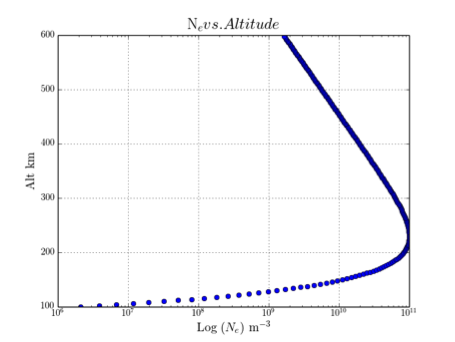
\includegraphics[width=3in]{nevsalt}
	\caption{Simulated electron density verses altitude.}	
	\label{fig:nevsalt}
\end{figure}

\begin{figure}
	\centering
	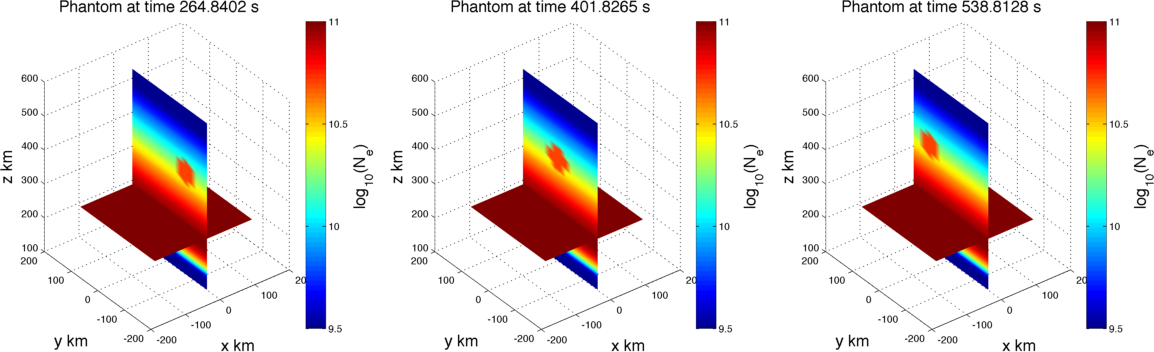
\includegraphics[width=6in]{phantom}
	\caption{Pmages from phantom.}	
	\label{fig:phantom}
\end{figure}

%In order to demonstrate the efficacy of the proposed framework, we consider a simplifying case corresponding to conditions expected in the polar cap ionosphere under southward IMF conditions. Specifically, we consider a structure density field translating at a constant convection velocity, where variations in the underlying potential field occur over scales that are large compared to radar FOV

The first example is a simple case of a small plasma enhancement moving through the radar field of view. This case is meant to model conditions expected in the polar cap ionosphere under southward IMF conditions \citep{Dahlgren:2012dq}. The background electron density varies in altitude as a Chapman function, shown in Figure \ref{fig:nevsalt}, while the electron and ion temperature remains constant. 

Embedded in the background there is a 35 km radius sphere of enhanced electron density of $5\times 10^{10} $ m$^{-3}$ centered at 400 km altitude moving at 500 m/s along the $\mathbf{y}$ direction. Images from this phantom can be seen in Figure \ref{fig:phantom}. To simplify the simulation the atmosphere is assumed to be 100\% Oxygen ions. For the ease of comparison the phantom is only shown in areas where it is in the radar's field of view. The positions of the 121 beam used for this case can be seen in Figure \ref{fig:beampattern}. 

Because only the electron density is varying the fitting method becomes simply a power estimate as the electron density is directly proportional to the return power if the temperature ration is known. This example allows the blurring from the space-time ambiguity function can be observed easier, while also showing trade offs between statistical variance and blurring. \footnote{I think we had a better way of stating this. }

Using the phantom we can see how just simply changing the integration time can impact the reconstruction. In Figure \ref{fig:variable} we can see a case were only 10 pulses are used for the reconstruction,which corresponds to an integration time of about 9 seconds. The enhancement can be seen as it moves through the field of view although there is that there is a high amount of variance in the reconstruction. Figure \ref{fig:blurred} shows the reconstruction with 200 pulses, 3 minute integration time. The variability has been reduced but there is a large amount of blurring of the enhancement as it moves through the field of view. % make variance measurement plots


\begin{figure}
	\centering
	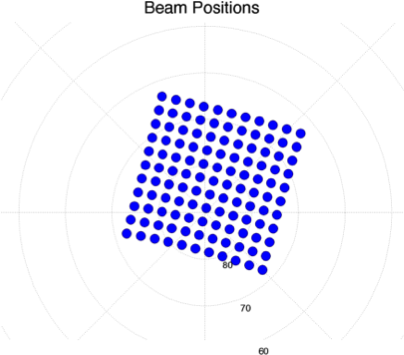
\includegraphics[width=3in]{beampattern}
	\caption{Radar beam pattern used in the simulations}	
	\label{fig:beampattern}
\end{figure}

\begin{figure}
	\centering
	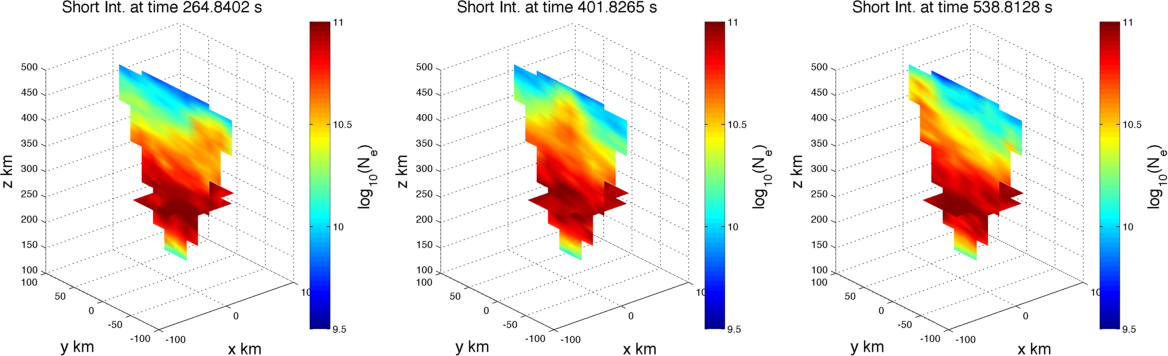
\includegraphics[width=6in]{variabledata}
	\caption{Reconstructions of $N_e$ using 10 Pulses.}	
	\label{fig:variable}
\end{figure}


\begin{figure}
	\centering
	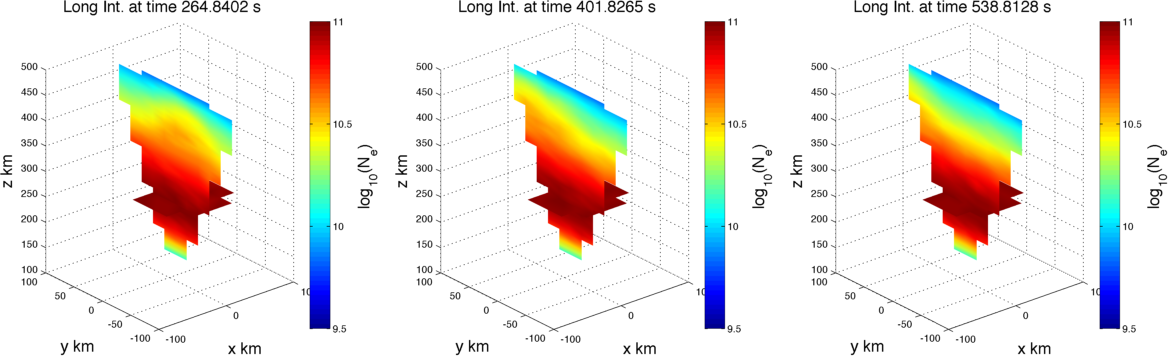
\includegraphics[width=6in]{blurreddata}
	\caption{Reconstructions of $N_e$ using 200 Pulses.}	
	\label{fig:blurred}
\end{figure}

In order to give a comparison based on integration time a phantom was also created one with no motion. This can be seen in the first pane Figure \ref{fig:statreconstruct}. An image using the same integration time as in Figure \ref{fig:variable} for the stationary phantom is the center pane in Figure \ref{fig:statreconstruct}. Another image using the longer integration time can be seen in right pane of Figure \ref{fig:statreconstruct}. These images show that the blurring is on the same order between both integration times.

\begin{figure}
	\centering
	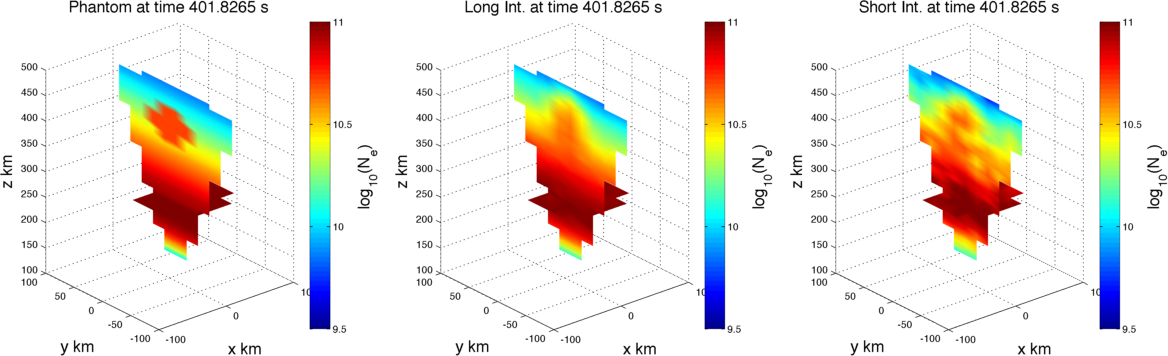
\includegraphics[width=6in]{stationary}
	\caption{Stationary phantom of $N_e$ along with reconstructions using 10 and 200 pulses.}	
	\label{fig:statreconstruct}
\end{figure}

\subsection{Case 2}
Secondly, we show results of a simulation of the plasma density enhancement through the field of view but the ion and electron temperatures are allowed to vary. This case will represent a departure from the standard blurring problem seen in image processing because the parameters to be estimated are related to the data through a non-linear expression. The resulting ACF estimates though are created through a linear blurring kernel in both time and space. 

We again use a plasma enhancement moving through the field of view at 500 m/s but the electron and ion temperature varies with time and altitude. The the background ion and electron temperature vs. height can be seen in Figure \ref{fig:allparamsphantom}. As the electron density enhancement travels through the field of view the temperatures drop by the same ratio that the electron density is enhanced. This is done to keep the variance the same. %check that


\begin{figure}
	\centering
	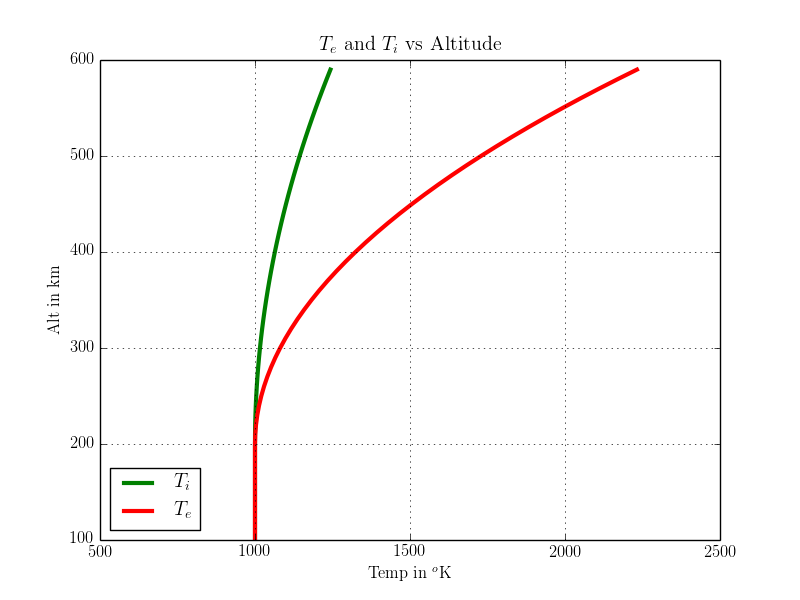
\includegraphics[width=4in]{tempvsheight}
	\caption{Ion \& electron temperature verses height for simulation. }	
	\label{fig:allparamsphantom}
\end{figure}

The phantoms for each parameter at approximately 402 seconds can be seen in Figure \ref{fig:allparamsphantom}. The reconstruction of this field at the same time can be seen in Figure \ref{fig:allparamsblurreddata}. The reconstruction does not seem to show the electron density enhancement even in a blurred form. 

\begin{figure}
	\centering
	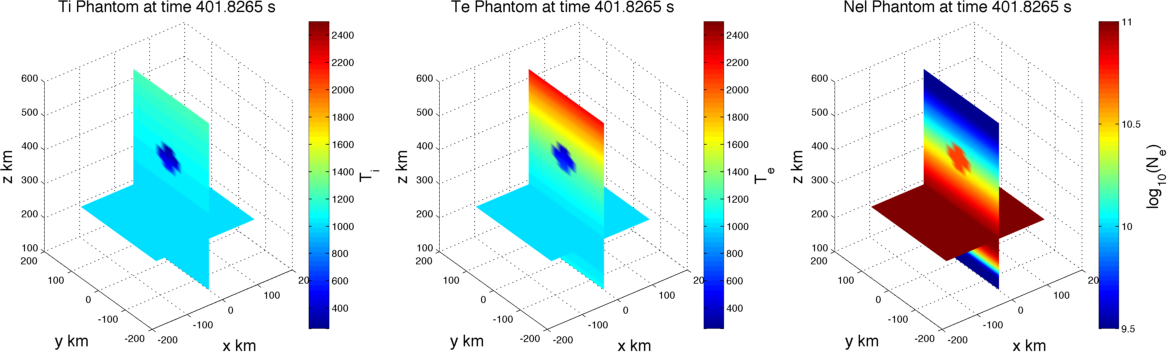
\includegraphics[width=6in]{allparamsphantom}
	\caption{Phantoms of $T_i$, $T_e$ and $N_e$ at $t=401.8265$s.}	
	\label{fig:allparamsphantom}
\end{figure}

\begin{figure}
	\centering
	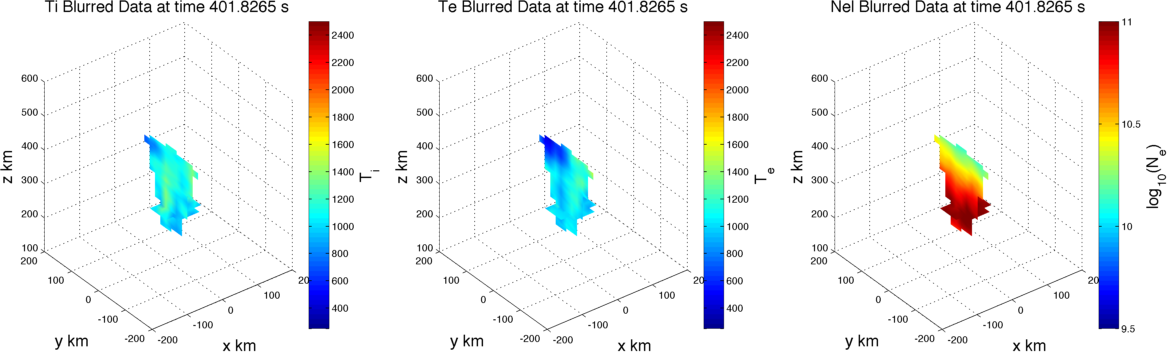
\includegraphics[width=6in]{allparamsblurreddata}
	\caption{Interpolated reconstructions of $T_i$, $T_e$ and $N_e$ at $t=401.8265$s.}	
	\label{fig:allparamsblurreddata}
\end{figure}

In order to determine the reason behind the poor reconstruction we look at the fit surface of one of the points in the reconstruction. The fit surface is the error between the estimated ISR spectrum and the spectrum derived from the different parameters. Comparing the points $\mathbf{r}=[10,10, 400]$km and the closest reconstruction point in the radar field of view, $\mathbf{r}_s=[6.72,1.80, 398.77]$. The time was chosen so the integrated measurement would be centered over the time when the enhancement moved through this point. During this time period the radar will integrate over two distributions of plasma at this point. The plasma at point $\mathbf{r}$ are $N_e=1.96\times 10^{10}$m$^{-3}$, $T_i =1064$ $^\circ$K and $T_e =1324$ $^\circ$K when there is no enhancement traveling through. When the enhancement is traveling through this point $N_e=5\times 10^{10}$m$^{-3}$, $T_i =416$ $^\circ$K and $T_e =518$ $^\circ$K. The speed of the enhancement, which is going at 500 m/s, causes about two-thirds of the pulses to correspond to the enhanced plasma during the integration.

The fit results in the parameter values at $\mathbf{r}$ are $N_e=2.36\times 10^{10}$m$^{-3}$, $T_i =973$ $^\circ$K and $T_e =500$ $^\circ$K. The fit surface was formed over the parameter space of $N_e$ $1\times 10^{10}$ to $1\times10^{11} $m$^{-3}$, and for both $T_e$ and $T_i$ were over an values 100 to 1500 $^\circ$K. In this case the fit surface showed that the global minimum was located in the same found in the same location as found by the Levenberg-Marquart algorithm. . A two dimensional cut of the fit surface at $N_e=2.43\times 10^{10} $ and showing its variability between $T_i$ and $T_e$ in Figure \ref{fig:fitsurface}. Since this is a global minimum supports the possibility of the non uniformity of the plasma parameters causing and erroneous fit. Mixtures of different plasma populations causing erroneous fits have been shown before such as in \citep{knudsen1993}. \footnote{Feel like I need a better ending to this section.}

\begin{figure}
	\centering
	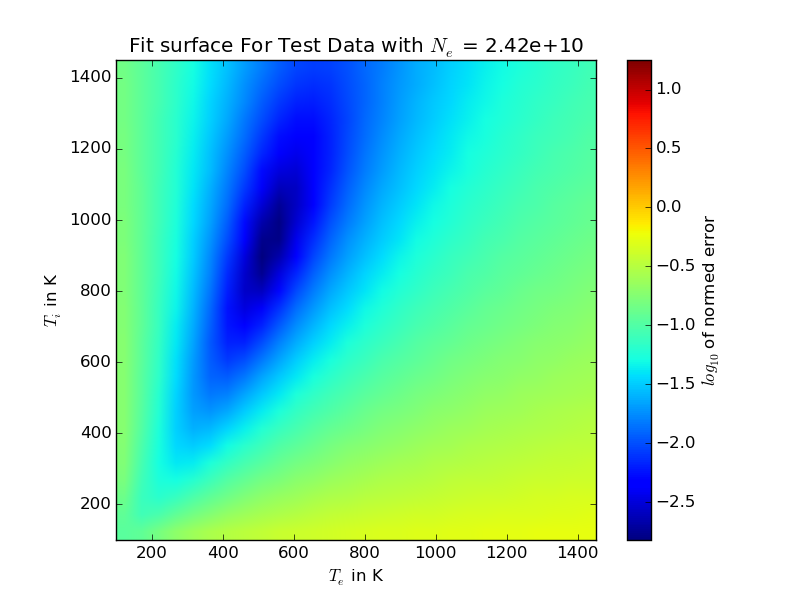
\includegraphics[width=6in]{Fitsurface3}
	\caption{fit surface.}	
	\label{fig:fitsurface}
\end{figure}

The spectrums that are yielded from the parameters along with what was estimated can be seen in Figure \ref{fig:spectrums}. In this case it can be seen that the spectrum estimated from the data has been reduced by the averaging over time and space which has lowered its power dramatically thus making it more similar to a spectrum with the improper values.\footnote{Gotta work on the wording here on my end. I can also grab other examples if need be.}
\begin{figure}
	\centering
	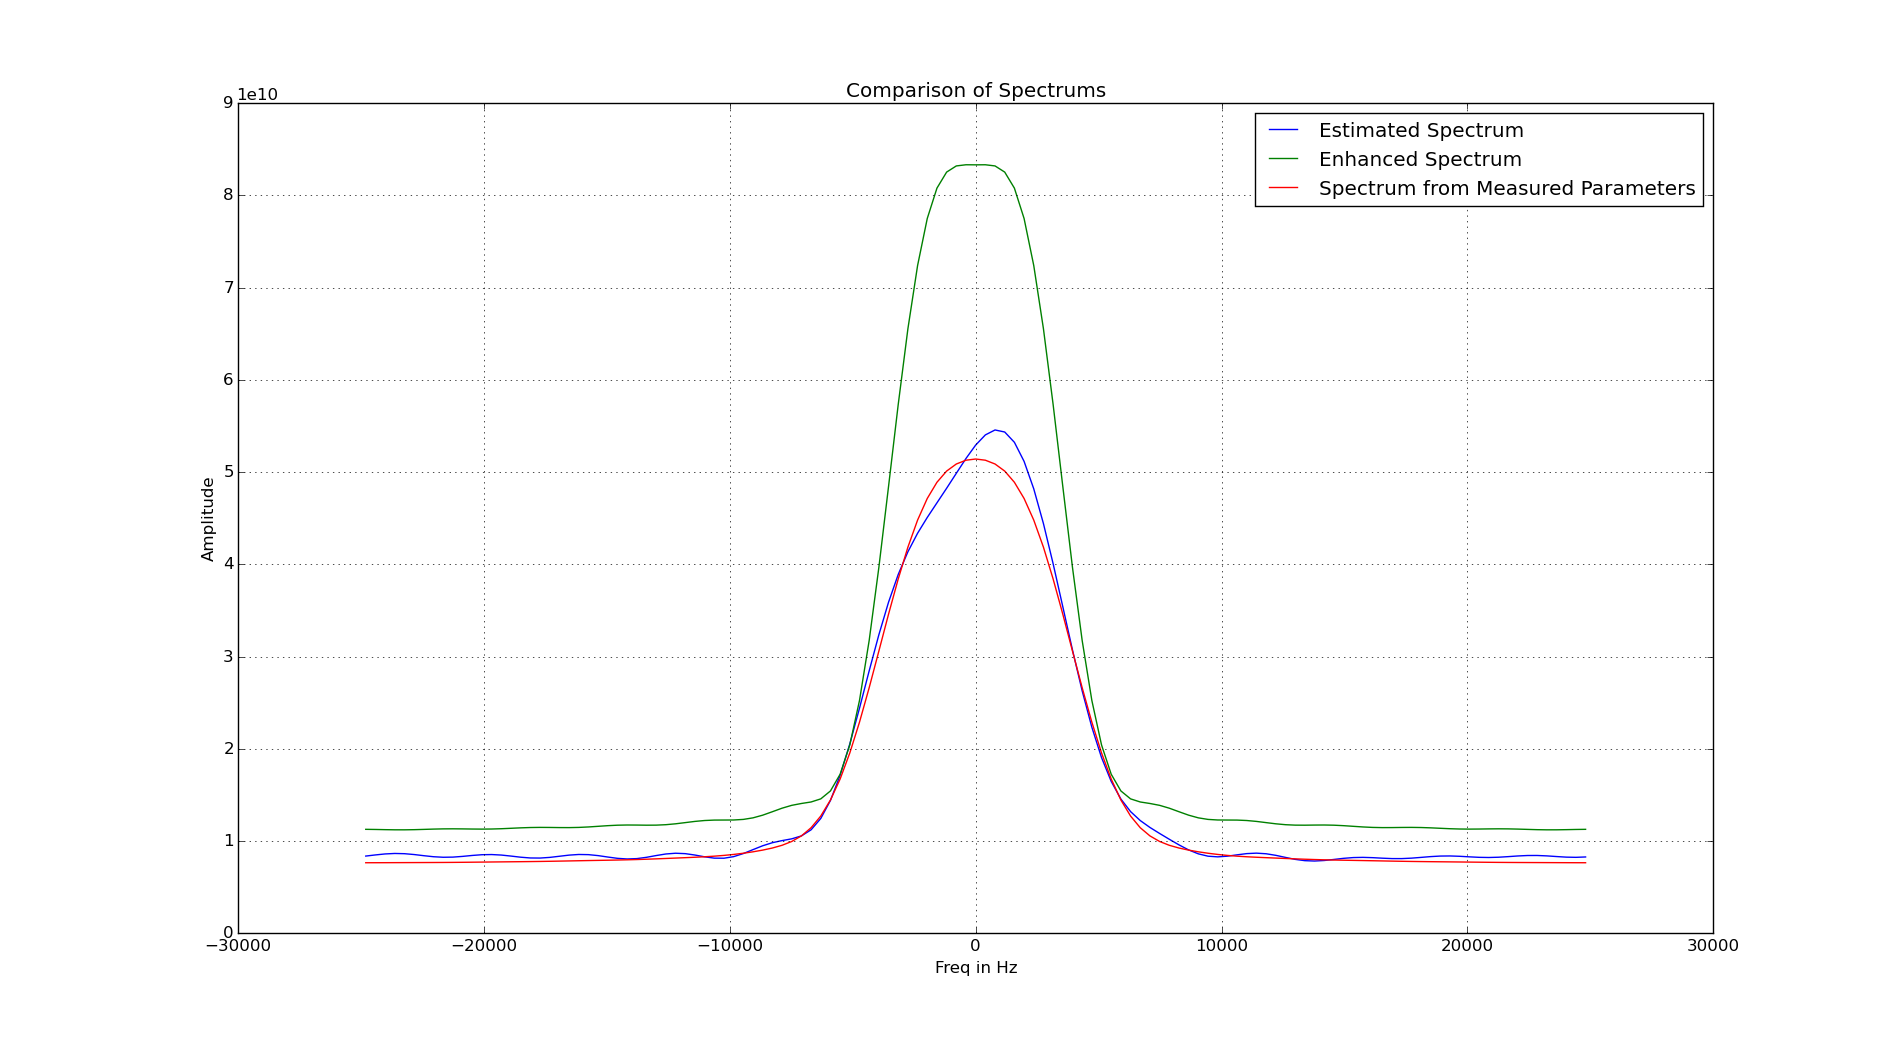
\includegraphics[width=6in]{spectrums}
	\caption{spectrums.}	
	\label{fig:spectrums}
\end{figure}
%%%%%%%%%%%%%% Mitigation %%%%%%%%%%%%%%%%%%%%%%%%%%%%%%%%%%%%%

\section{Possible Mitigation Techniques}

As can be seen from the previous sections a number of different types of errors can occur due to this type of space-time ambiguity function. There are a number of possible approaches one could take in order to produce an improved data product from electronically scanned ISR measurements. This discussion isn't meant to be exhaustive but give an idea of the utility of this frame work. In order to focus this section we will concentrate on methods to remove motion blur type errors that occur when plasma is moving through the field of view, and techniques to improve the spatio-temporal resolution of the measurements.% and better ways to interpolate measurements.

In order to reduce the impact from plasma parcel motion, a relatively simple approach would involve processing the data in the frame of reference of the moving density field. The convection velocity is manifested as a bulk Doppler shift in the ISR spectrum.Under the assumptions applied in our examples, this Doppler shift is independent of the other parameters, and so $\mathbf{v}$ in Equation \ref{eqn:L5}  could be extracted using the analysis described by \citet{RDS:RDS5552} and \citet{butler:imagingfregiondrifts}. After measuring the velocity instead of integrating in the same beam one could integrate across different beams using this knowledge. This would allow for ACF to be formed from the same populations of plasma as it moves through the field of view.

If one wants to improve the resolution of the the plasma parameters it may be necessary to do some sort of regularization. There are two type of regularization that can be applied in this case the first is parameter based regularization, like full profile analysis \citet{RDS:RDS3308,hysell2008}. We will use the term parameter based regularization in this case means applying constraints to the physical parameters that are often determined after fitting. This can require a large amount of calculation because the fitting and constraints are done in one step. Currently full profile analysis has only been applied along the range dimension and not in all three spatial dimensions. Still if full profile analysis is to be extended so it can be used in ESA systems a forward model between the actual ACF and the one measured in the radar would be needed. This is encompassed within Equation \ref{eqn:sptamb}.  

The other method we will refer to as data based regularization. This term infers the application of constraints to the estimates of the autocorrelation functions and then fitting . The constraints usually deal with how the data changes over time and space by constraining the energy of the ACFs \citep{Virtanen:2008vx, nikoukar2008} or its derivative \citep{nikoukar:thesis}. A simplification of the data based regularization is that one is doing a deconvolution operation on the ACFs. This has an advantage that one can use linear inverse theory to estimate to do the reconstruction, unlike with parameter based regularization schemes such as full profile analysis. Because of this data based regularization has the advantage of generally being more computationally tractable then parameter based. One of the drawbacks though with data based regularization though is that is very difficult to argue what constraint would be "correct" to use. While in full profile analysis the constraints are based on known physics in the ionosphere to create a measurement. In any case in order to extend the methodology from \citet{Virtanen:2008vx} and \citet{ nikoukar2008} one can use the kernel $L$ if trying to improve the measurements from an ESA ISR. %Using the ideas stated in this paper one can cast the reconstruction of the four dimensional function of the ACFs in these terms. The issue with doing this data based reconstruction is it is unknown how to constrain the reconstruction in the best way. 


%The two examples of data based regularization in the one dimensions ISR literature are lag profile inversion and deconvolution methods. Lag profile inversion creates an operator that takes the measured data from a theoretical ACFs to the measured ACFs \citep{Virtanen:2008vx}. Along with the operator there is also an assumed Gaussian error. This error can be then estimated from the data. This Bayesian frame work can actually be rewritten as a least squares minimization along with a Tikhonov constraint. Because of this one can show that the deconvolution methods from \citet{nikoukar2008} are extremely similar to lag profile inversion with differences in only what type of constraints are used.

%In order to improve the resolution of ESA ISR measurements regularization methods have advantages and disadvantages. In data based regularization constraints must be applied to the ACFs, which yields the question of what is the most reasonable constraint to use. Although this methodology will allow researchers to use methods from linear inverse theory, which has been well studied. The parameter based regularization method allows for use of physics based constraints to reconstruct the parameters. This technique though would likely yield solutions that would be very computationally intensive compared to techniques for data based regularization. In any case, both methods requires the forward model which has been discussed in this paper.
%With this in mind one can go a step further and investigate super resolution methods seen in image processing literature \citep{Takeda:2009ep},\citep{Takeda:2011en}. With these techniques along with the data regularization based frame work in one dimensional ISR these techniques could be used to reconstruct the ACFs. This would require a complete change in the methodology in which 3-D ISR data is investigated. Basically instead of fitting data in the coordinate space of the radar we would first re-grid the data in a Cartesian space and then apply the nonlinear fitting. This would have the advantage of working with a linear inverse problem but the issues would be the same as with other data based regularization techniques were there is a question of what type of constraint should be used as opposed to a straight forward physical constraint. 
%%%%%%%%%%%%%% Conclusion %%%%%%%%%%%%%%%%%%%%%%%%%%%%%%%%%%%%

\section{Conclusion}This publication has laid the foundation for the optimal analysis of volumetric data acquired from electronically steerable ISR systems. This framework allows for taking into account the antenna beam pattern, pulse pattern and time integration. Through simulation we have shown how plasma motion can impact reconstruction of parameters which compounded with the non-linear nature of the parameter fitting step can create errors which are hard to predict. Lastly we briefly outlined a number of possible approaches improving measurements derived from ESA ISRs.%estimating parameter fields at higher spatio-temporal resolutions than what is currently possible.


\appendix
\section{Derivation of Idealized AMISR Array Pattern} \label{App:AMISRarr}
The current antenna on the AMISR systems is made up 8x16 set of panel of half wave cross dipoles. Each panel has 32 cross dipoles in a 8x4 hexagonal configuration. In the current set up at the Poker Flat site this yields at 4096 element array in a 64x64 element hexagonal configuration.

In order to simplify the antenna can be treated as two rectangular arrays of cross dipoles interleaved together. In the $x$ direction each of these arrays will have a spacing of $2d_x$ with $M/2$ elements. The $y$ direction will be of length $N$ elements and spacing $d_y$. Using basic planar phase array theory, \citep{Balanis:2005:ATA:1208379}, we can start with the linear array pattern from the first array can be represented as 

\begin{equation}
\label{eqn:arrpat1}
E_1(\theta,\phi) =\displaystyle \sum_{m=1}^{M/2}\sum_{n=1}^{N} e^{-j2\left(m-1\right)kd_x\sin\theta\cos\phi -j\left(n-1\right) k d_y\sin\theta\sin\phi}.
\end{equation}

\noindent Since the second array can be though of a shifted version of the first in the $x$ direction we get the following

\begin{equation}
\label{eqn:arrpat2}
E_2(\theta,\phi) =\displaystyle \sum_{m=1}^{M/2}\sum_{n=1}^{N} e^{-j\left(2m-1\right)kd_x\sin\theta\cos\phi -j\left(n-1/2\right) k d_y\sin\theta\sin\phi}.
\end{equation}

In order to simplify notation we will make the following substitutions, $\psi_x = -k d_x\sin\theta\cos\phi$, $\psi_y = -k d_y\sin\theta\sin\phi$. Using Equations \ref{eqn:arrpat1} and \ref{eqn:arrpat2} we can see the following relationship,

\begin{equation}
\label{eqn:arrpateqn}
E_2(\theta,\phi)  = e^{j(\psi_y/2 + \psi_x)} E_1(\theta,\phi)  = \displaystyle \sum_{m=1}^{M/2}\sum_{n=1}^{N} e^{-j2\left(m-1\right) \psi_x -j\left(n-1\right) \psi_y}.
\end{equation}

\noindent Adding $E_1$ and $E_2$ together we get the following linear array pattern

\begin{equation} \label{eq1}
\begin{split}
E(\theta,\phi) &= \displaystyle  \left(1+e^{j(\psi_y/2 + \psi_x)}\right)\sum_{m=1}^{M/2}\sum_{n=1}^{N} e^{-j2\left(m-1\right) \psi_x -j\left(n-1\right) \psi_y}.\\
& = \frac{1}{MN} \left(1+e^{j(\psi_y/2 + \psi_x)}\right)\frac{\sin((M/2) \psi_x)}{\sin(\psi_x)} \frac{\sin((N/2) \psi_x)}{\sin(\psi_x/2)}.
\end{split}
\end{equation}

Since the array is steerable this can be taken into account in the equations by simply changing the definitions of $\psi_x $ and $\psi_y$ to $\psi_x = k d_x(\sin\theta\cos\phi-\sin\theta_s\cos\phi_s)$, and $\psi_y = k d_y(\sin\theta\sin\phi-\sin\theta_s\sin\phi_s)$. Lastly the antenna pattern of a single cross dipole can be represented as $ \frac{1}{2}(1+\cos^2(\theta))$\citep{Balanis:2005:ATA:1208379}. By taking the squared magnitude of the array factor and multiplying it with the pattern of the dipole we get Equation \ref{eqn:amisrpat},

\begin{equation}
\label{eqn:amisrpatfinal}
F(\theta_s,\phi_s,\theta,\phi) = \frac{1}{2}(1+\cos(\theta)^2)\left| \frac{1}{MN} \left(1+e^{j(\psi_y/2 + \psi_x)}\right)\frac{\sin((M/2) \psi_x)}{\sin(\psi_x)} \frac{\sin((N/2) \psi_x)}{\sin(\psi_x/2)}\right|^2.
\end{equation}
 
\bibliographystyle{BibTeX/agufull08}
\bibliography{BibTeX/litreview}

\begin{acknowledgments}
(Text here)
\end{acknowledgments}

\end{article}

\end{document}